% Options for packages loaded elsewhere
\PassOptionsToPackage{unicode}{hyperref}
\PassOptionsToPackage{hyphens}{url}
%
\documentclass[
]{book}
\usepackage{amsmath,amssymb}
\usepackage{lmodern}
\usepackage{iftex}
\ifPDFTeX
  \usepackage[T1]{fontenc}
  \usepackage[utf8]{inputenc}
  \usepackage{textcomp} % provide euro and other symbols
\else % if luatex or xetex
  \usepackage{unicode-math}
  \defaultfontfeatures{Scale=MatchLowercase}
  \defaultfontfeatures[\rmfamily]{Ligatures=TeX,Scale=1}
\fi
% Use upquote if available, for straight quotes in verbatim environments
\IfFileExists{upquote.sty}{\usepackage{upquote}}{}
\IfFileExists{microtype.sty}{% use microtype if available
  \usepackage[]{microtype}
  \UseMicrotypeSet[protrusion]{basicmath} % disable protrusion for tt fonts
}{}
\makeatletter
\@ifundefined{KOMAClassName}{% if non-KOMA class
  \IfFileExists{parskip.sty}{%
    \usepackage{parskip}
  }{% else
    \setlength{\parindent}{0pt}
    \setlength{\parskip}{6pt plus 2pt minus 1pt}}
}{% if KOMA class
  \KOMAoptions{parskip=half}}
\makeatother
\usepackage{xcolor}
\usepackage{color}
\usepackage{fancyvrb}
\newcommand{\VerbBar}{|}
\newcommand{\VERB}{\Verb[commandchars=\\\{\}]}
\DefineVerbatimEnvironment{Highlighting}{Verbatim}{commandchars=\\\{\}}
% Add ',fontsize=\small' for more characters per line
\usepackage{framed}
\definecolor{shadecolor}{RGB}{248,248,248}
\newenvironment{Shaded}{\begin{snugshade}}{\end{snugshade}}
\newcommand{\AlertTok}[1]{\textcolor[rgb]{0.94,0.16,0.16}{#1}}
\newcommand{\AnnotationTok}[1]{\textcolor[rgb]{0.56,0.35,0.01}{\textbf{\textit{#1}}}}
\newcommand{\AttributeTok}[1]{\textcolor[rgb]{0.77,0.63,0.00}{#1}}
\newcommand{\BaseNTok}[1]{\textcolor[rgb]{0.00,0.00,0.81}{#1}}
\newcommand{\BuiltInTok}[1]{#1}
\newcommand{\CharTok}[1]{\textcolor[rgb]{0.31,0.60,0.02}{#1}}
\newcommand{\CommentTok}[1]{\textcolor[rgb]{0.56,0.35,0.01}{\textit{#1}}}
\newcommand{\CommentVarTok}[1]{\textcolor[rgb]{0.56,0.35,0.01}{\textbf{\textit{#1}}}}
\newcommand{\ConstantTok}[1]{\textcolor[rgb]{0.00,0.00,0.00}{#1}}
\newcommand{\ControlFlowTok}[1]{\textcolor[rgb]{0.13,0.29,0.53}{\textbf{#1}}}
\newcommand{\DataTypeTok}[1]{\textcolor[rgb]{0.13,0.29,0.53}{#1}}
\newcommand{\DecValTok}[1]{\textcolor[rgb]{0.00,0.00,0.81}{#1}}
\newcommand{\DocumentationTok}[1]{\textcolor[rgb]{0.56,0.35,0.01}{\textbf{\textit{#1}}}}
\newcommand{\ErrorTok}[1]{\textcolor[rgb]{0.64,0.00,0.00}{\textbf{#1}}}
\newcommand{\ExtensionTok}[1]{#1}
\newcommand{\FloatTok}[1]{\textcolor[rgb]{0.00,0.00,0.81}{#1}}
\newcommand{\FunctionTok}[1]{\textcolor[rgb]{0.00,0.00,0.00}{#1}}
\newcommand{\ImportTok}[1]{#1}
\newcommand{\InformationTok}[1]{\textcolor[rgb]{0.56,0.35,0.01}{\textbf{\textit{#1}}}}
\newcommand{\KeywordTok}[1]{\textcolor[rgb]{0.13,0.29,0.53}{\textbf{#1}}}
\newcommand{\NormalTok}[1]{#1}
\newcommand{\OperatorTok}[1]{\textcolor[rgb]{0.81,0.36,0.00}{\textbf{#1}}}
\newcommand{\OtherTok}[1]{\textcolor[rgb]{0.56,0.35,0.01}{#1}}
\newcommand{\PreprocessorTok}[1]{\textcolor[rgb]{0.56,0.35,0.01}{\textit{#1}}}
\newcommand{\RegionMarkerTok}[1]{#1}
\newcommand{\SpecialCharTok}[1]{\textcolor[rgb]{0.00,0.00,0.00}{#1}}
\newcommand{\SpecialStringTok}[1]{\textcolor[rgb]{0.31,0.60,0.02}{#1}}
\newcommand{\StringTok}[1]{\textcolor[rgb]{0.31,0.60,0.02}{#1}}
\newcommand{\VariableTok}[1]{\textcolor[rgb]{0.00,0.00,0.00}{#1}}
\newcommand{\VerbatimStringTok}[1]{\textcolor[rgb]{0.31,0.60,0.02}{#1}}
\newcommand{\WarningTok}[1]{\textcolor[rgb]{0.56,0.35,0.01}{\textbf{\textit{#1}}}}
\usepackage{longtable,booktabs,array}
\usepackage{calc} % for calculating minipage widths
% Correct order of tables after \paragraph or \subparagraph
\usepackage{etoolbox}
\makeatletter
\patchcmd\longtable{\par}{\if@noskipsec\mbox{}\fi\par}{}{}
\makeatother
% Allow footnotes in longtable head/foot
\IfFileExists{footnotehyper.sty}{\usepackage{footnotehyper}}{\usepackage{footnote}}
\makesavenoteenv{longtable}
\usepackage{graphicx}
\makeatletter
\def\maxwidth{\ifdim\Gin@nat@width>\linewidth\linewidth\else\Gin@nat@width\fi}
\def\maxheight{\ifdim\Gin@nat@height>\textheight\textheight\else\Gin@nat@height\fi}
\makeatother
% Scale images if necessary, so that they will not overflow the page
% margins by default, and it is still possible to overwrite the defaults
% using explicit options in \includegraphics[width, height, ...]{}
\setkeys{Gin}{width=\maxwidth,height=\maxheight,keepaspectratio}
% Set default figure placement to htbp
\makeatletter
\def\fps@figure{htbp}
\makeatother
\setlength{\emergencystretch}{3em} % prevent overfull lines
\providecommand{\tightlist}{%
  \setlength{\itemsep}{0pt}\setlength{\parskip}{0pt}}
\setcounter{secnumdepth}{5}
\usepackage{booktabs}
\ifLuaTeX
  \usepackage{selnolig}  % disable illegal ligatures
\fi
\usepackage[]{natbib}
\bibliographystyle{plainnat}
\IfFileExists{bookmark.sty}{\usepackage{bookmark}}{\usepackage{hyperref}}
\IfFileExists{xurl.sty}{\usepackage{xurl}}{} % add URL line breaks if available
\urlstyle{same} % disable monospaced font for URLs
\hypersetup{
  pdftitle={Portfolio},
  pdfauthor={Dian Dupon},
  hidelinks,
  pdfcreator={LaTeX via pandoc}}

\title{Portfolio}
\author{Dian Dupon}
\date{2023-05-21}

\begin{document}
\maketitle

{
\setcounter{tocdepth}{1}
\tableofcontents
}
\hypertarget{about}{%
\chapter{About}\label{about}}

This is a \emph{sample} book written in \textbf{Markdown}. You can use anything that Pandoc's Markdown supports; for example, a math equation \(a^2 + b^2 = c^2\).

\hypertarget{usage}{%
\section{Usage}\label{usage}}

Each \textbf{bookdown} chapter is an .Rmd file, and each .Rmd file can contain one (and only one) chapter. A chapter \emph{must} start with a first-level heading: \texttt{\#\ A\ good\ chapter}, and can contain one (and only one) first-level heading.

Use second-level and higher headings within chapters like: \texttt{\#\#\ A\ short\ section} or \texttt{\#\#\#\ An\ even\ shorter\ section}.

The \texttt{index.Rmd} file is required, and is also your first book chapter. It will be the homepage when you render the book.

\hypertarget{render-book}{%
\section{Render book}\label{render-book}}

You can render the HTML version of this example book without changing anything:

\begin{enumerate}
\def\labelenumi{\arabic{enumi}.}
\item
  Find the \textbf{Build} pane in the RStudio IDE, and
\item
  Click on \textbf{Build Book}, then select your output format, or select ``All formats'' if you'd like to use multiple formats from the same book source files.
\end{enumerate}

Or build the book from the R console:

\begin{Shaded}
\begin{Highlighting}[]
\NormalTok{bookdown}\SpecialCharTok{::}\FunctionTok{render\_book}\NormalTok{()}
\end{Highlighting}
\end{Shaded}

To render this example to PDF as a \texttt{bookdown::pdf\_book}, you'll need to install XeLaTeX. You are recommended to install TinyTeX (which includes XeLaTeX): \url{https://yihui.org/tinytex/}.

\hypertarget{preview-book}{%
\section{Preview book}\label{preview-book}}

As you work, you may start a local server to live preview this HTML book. This preview will update as you edit the book when you save individual .Rmd files. You can start the server in a work session by using the RStudio add-in ``Preview book'', or from the R console:

\begin{Shaded}
\begin{Highlighting}[]
\NormalTok{bookdown}\SpecialCharTok{::}\FunctionTok{serve\_book}\NormalTok{()}
\end{Highlighting}
\end{Shaded}

\hypertarget{c.-elegans-offspring-count-with-different-components}{%
\chapter{C. elegans offspring count with different components''}\label{c.-elegans-offspring-count-with-different-components}}

\hypertarget{installing-packages}{%
\section{Installing packages}\label{installing-packages}}

\begin{Shaded}
\begin{Highlighting}[]
\CommentTok{\# install.packages("gitcreds")}
\CommentTok{\# library(gitcreds)}
\CommentTok{\# gitcreds\_set()}
\end{Highlighting}
\end{Shaded}

\hypertarget{importing-the-data}{%
\section{\texorpdfstring{Importing the data }{Importing the data  }}\label{importing-the-data}}

For this experiment the data from the CE.LIQ.FLOW.062\_Tidydata.xlsx file was used to determine the effect of compound concentrations on offspring count and whether the different compounds have a positive effect on the amount of offspring.
After importing the data, the data types of columns were checked to see if these were correctly assigned.

\begin{Shaded}
\begin{Highlighting}[]
\CommentTok{\# Loading library}
\FunctionTok{library}\NormalTok{(tidyverse)}
\FunctionTok{library}\NormalTok{(readxl)}

\CommentTok{\# Getting the data from the downloaded Excel file}
\CommentTok{\# You can find the raw data in the Data\_raw folder of this experiment}
\NormalTok{elegans\_data }\OtherTok{\textless{}{-}} \FunctionTok{read\_excel}\NormalTok{(}\StringTok{"\textasciitilde{}/DSFB2/dsfb2\_workflows\_portfolio/Portfolio/C.elegans\_experiment/Data\_raw/CE.LIQ.FLOW.062\_Tidydata.xlsx"}\NormalTok{)}

\CommentTok{\# Check if the data imported correctly}
\FunctionTok{head}\NormalTok{(elegans\_data)}
\end{Highlighting}
\end{Shaded}

\begin{verbatim}
## # A tibble: 6 x 34
##   plateRow plateColumn vialNr dropCode expType    expReplicate expName        
##   <lgl>    <lgl>        <dbl> <chr>    <chr>             <dbl> <chr>          
## 1 NA       NA               1 a        experiment            3 CE.LIQ.FLOW.062
## 2 NA       NA               1 b        experiment            3 CE.LIQ.FLOW.062
## 3 NA       NA               1 c        experiment            3 CE.LIQ.FLOW.062
## 4 NA       NA               1 d        experiment            3 CE.LIQ.FLOW.062
## 5 NA       NA               1 e        experiment            3 CE.LIQ.FLOW.062
## 6 NA       NA               2 a        experiment            3 CE.LIQ.FLOW.062
## # i 27 more variables: expDate <dttm>, expResearcher <chr>, expTime <dbl>,
## #   expUnit <chr>, expVolumeCounted <dbl>, RawData <dbl>, compCASRN <chr>,
## #   compName <chr>, compConcentration <chr>, compUnit <chr>,
## #   compDelivery <chr>, compVehicle <chr>, elegansStrain <chr>,
## #   elegansInput <dbl>, bacterialStrain <chr>, bacterialTreatment <chr>,
## #   bacterialOD600 <dbl>, bacterialConcX <dbl>, bacterialVolume <dbl>,
## #   bacterialVolUnit <chr>, incubationVial <chr>, incubationVolume <dbl>, ...
\end{verbatim}

\begin{Shaded}
\begin{Highlighting}[]
\CommentTok{\# Check data types of specific columns}
\FunctionTok{str}\NormalTok{(elegans\_data}\SpecialCharTok{$}\NormalTok{RawData)}
\end{Highlighting}
\end{Shaded}

\begin{verbatim}
##  num [1:360] 44 37 45 47 41 35 41 36 40 38 ...
\end{verbatim}

\begin{Shaded}
\begin{Highlighting}[]
\FunctionTok{str}\NormalTok{(elegans\_data}\SpecialCharTok{$}\NormalTok{compName)}
\end{Highlighting}
\end{Shaded}

\begin{verbatim}
##  chr [1:360] "2,6-diisopropylnaphthalene" "2,6-diisopropylnaphthalene" ...
\end{verbatim}

\begin{Shaded}
\begin{Highlighting}[]
\FunctionTok{str}\NormalTok{(elegans\_data}\SpecialCharTok{$}\NormalTok{compConcentration)}
\end{Highlighting}
\end{Shaded}

\begin{verbatim}
##  chr [1:360] "4.99" "4.99" "4.99" "4.99" "4.99" "4.99" "4.99" "4.99" "4.99" ...
\end{verbatim}

The data type of the column compConcentration has not been correctly assigned during the importing of the data into R. Therefore we need to change the data type of this column.

\begin{Shaded}
\begin{Highlighting}[]
\CommentTok{\# Change column data type to numeric}
\NormalTok{elegans\_data\_tidy }\OtherTok{\textless{}{-}} \FunctionTok{transform}\NormalTok{(elegans\_data, }\AttributeTok{compConcentration =} \FunctionTok{as.numeric}\NormalTok{(compConcentration))}

\CommentTok{\# Check if it is correctly assigned}
\FunctionTok{str}\NormalTok{(elegans\_data\_tidy}\SpecialCharTok{$}\NormalTok{compConcentration)}
\end{Highlighting}
\end{Shaded}

\begin{verbatim}
##  num [1:360] 4.99 4.99 4.99 4.99 4.99 4.99 4.99 4.99 4.99 4.99 ...
\end{verbatim}

After making the data from the excel file tidy a scatterplot is created to study the data of the plate experiment more thoroughly.

\hypertarget{scatterplot-of-the-c.-elegans-plate-experiment}{%
\section{Scatterplot of the C. elegans plate experiment}\label{scatterplot-of-the-c.-elegans-plate-experiment}}

\begin{Shaded}
\begin{Highlighting}[]
\CommentTok{\# Load library}
\FunctionTok{library}\NormalTok{(ggplot2)}

\CommentTok{\# Creating the scatterplot}
\NormalTok{elegans\_data\_tidy }\SpecialCharTok{\%\textgreater{}\%} \FunctionTok{ggplot}\NormalTok{(}\FunctionTok{aes}\NormalTok{(}\AttributeTok{x=}\FunctionTok{log10}\NormalTok{(compConcentration}\FloatTok{+0.00005}\NormalTok{), }\AttributeTok{y=}\NormalTok{ RawData))}\SpecialCharTok{+} \CommentTok{\#Adding 0.0005 to prevent data loss}
  \FunctionTok{geom\_jitter}\NormalTok{(}\FunctionTok{aes}\NormalTok{(}\AttributeTok{colour=}\NormalTok{compName, }\AttributeTok{shape =}\NormalTok{ expType), }\AttributeTok{width =} \FloatTok{0.05}\NormalTok{)}\SpecialCharTok{+}
  \FunctionTok{theme\_bw}\NormalTok{()}\SpecialCharTok{+}
  \FunctionTok{labs}\NormalTok{(}\AttributeTok{title =} \StringTok{"C. elegans offspring count"}\NormalTok{, }\AttributeTok{x =} \StringTok{"Log 10 compound Concentration (nM)"}\NormalTok{, }\AttributeTok{y =} \StringTok{"C. elegans Counts"}\NormalTok{)}
\end{Highlighting}
\end{Shaded}

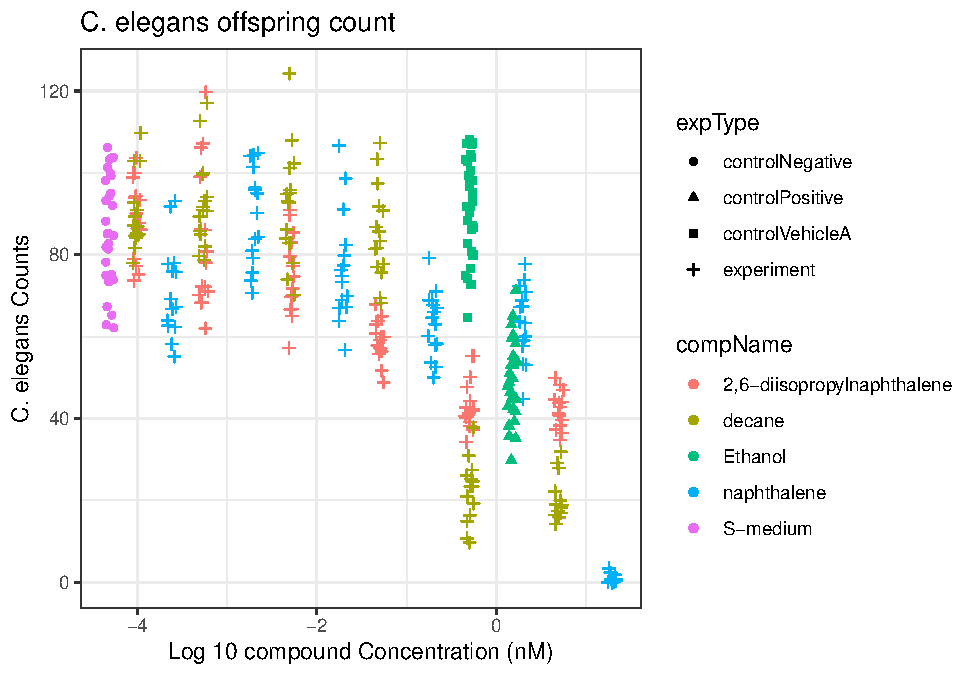
\includegraphics{_main_files/figure-latex/scatterplot-1.pdf}

The positive control for this experiment is ethanol. The negative control for this experiment is S-medium.

To analyse if there is indeed an effect of different concentrations on offspring count and whether the different compounds have a different curve it is advisable to make a dosis-response curve (IC50). To make this curve you need to follow the next few steps:
1. Normalize the data to the controlNegative condition.
2. Fit a dose-response curve to the data for each compound using a four-parameter logistic model.
3. Estimate the IC50 value for each compound based on the fitted curve.
4. Compare the IC50 values across the different compounds to see if there are any differences in growth of the C. elegans offspring.
5. Perform statistical tests to determine whether there is a significant effect of concentration on offspring count for each compound.

You want to normalize the data to ensure that any differences we observe in the data between the different compounds and concentrations are not simply due to differences in the overall baseline level of the response.

\hypertarget{normalizing-the-data}{%
\section{\texorpdfstring{Normalizing the data }{Normalizing the data  }}\label{normalizing-the-data}}

\begin{Shaded}
\begin{Highlighting}[]
\CommentTok{\# Calculate the normalization factor}
\NormalTok{norm\_factor }\OtherTok{\textless{}{-}} \FunctionTok{mean}\NormalTok{(elegans\_data\_tidy}\SpecialCharTok{$}\NormalTok{RawData[elegans\_data\_tidy}\SpecialCharTok{$}\NormalTok{expType }\SpecialCharTok{==} \StringTok{"controlNegative"}\NormalTok{])}

\CommentTok{\# Normalize the data}
\NormalTok{elegans\_data\_tidy}\SpecialCharTok{$}\NormalTok{Normalized }\OtherTok{\textless{}{-}}\NormalTok{ elegans\_data\_tidy}\SpecialCharTok{$}\NormalTok{RawData }\SpecialCharTok{/}\NormalTok{ norm\_factor}

\CommentTok{\# Setting the negative control value to 1}
\NormalTok{elegans\_data\_tidy}\SpecialCharTok{$}\NormalTok{Normalized[elegans\_data\_tidy}\SpecialCharTok{$}\NormalTok{expType }\SpecialCharTok{==} \StringTok{"Negative Control"}\NormalTok{] }\OtherTok{\textless{}{-}} \DecValTok{1}

\CommentTok{\# Creating the plot with the normalized data}
\NormalTok{elegans\_data\_tidy }\SpecialCharTok{\%\textgreater{}\%} \FunctionTok{ggplot}\NormalTok{(}\FunctionTok{aes}\NormalTok{(}\AttributeTok{x =} \FunctionTok{log10}\NormalTok{(compConcentration}\FloatTok{+0.00005}\NormalTok{), }\AttributeTok{y =}\NormalTok{ Normalized)) }\SpecialCharTok{+}
  \FunctionTok{geom\_jitter}\NormalTok{(}\FunctionTok{aes}\NormalTok{(}\AttributeTok{colour=}\NormalTok{ compName, }\AttributeTok{shape=}\NormalTok{ expType), }\AttributeTok{width =} \FloatTok{0.05}\NormalTok{)}\SpecialCharTok{+}
  \FunctionTok{labs}\NormalTok{(}\AttributeTok{title =} \StringTok{"Normalized C. elegans offspring count"}\NormalTok{, }\AttributeTok{x =} \StringTok{"Compound Concentration (nM)"}\NormalTok{, }\AttributeTok{y =} \StringTok{"Normalized C. elegans Counts"}\NormalTok{)}
\end{Highlighting}
\end{Shaded}

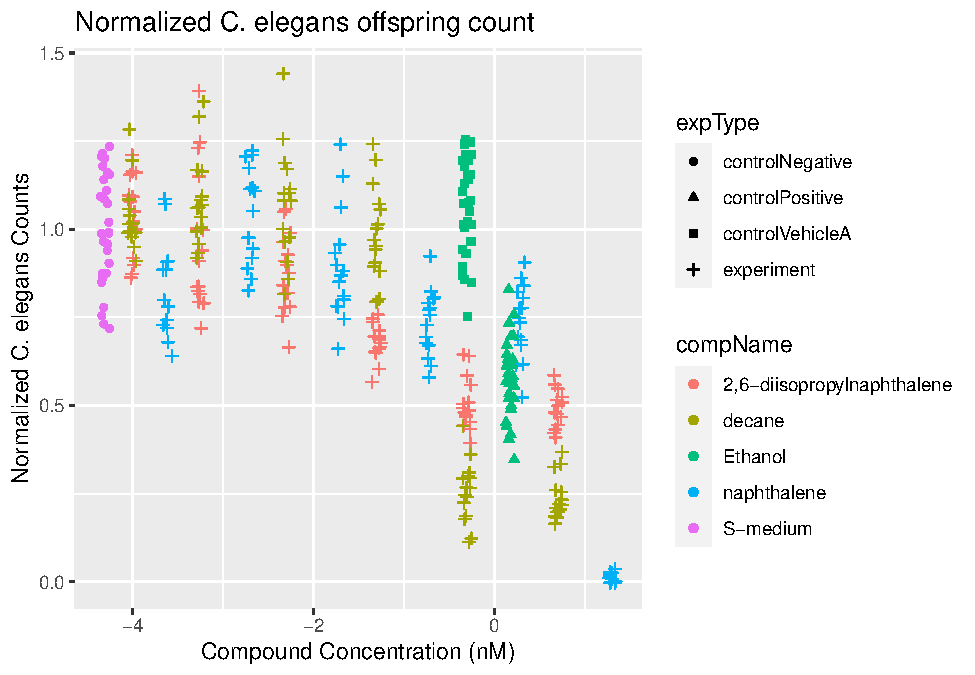
\includegraphics{_main_files/figure-latex/normalizing the data-1.pdf}

Based on the graphs above there can be concluded that 2.6-diisopropylnaphtalene, decane and nepthalene all cause a decrease in the amount of C. elegans offspring.

\hypertarget{scoring-a-publication-on-reproducibility}{%
\chapter{\texorpdfstring{Scoring a publication on reproducibility }{Scoring a publication on reproducibility  }}\label{scoring-a-publication-on-reproducibility}}

Often times the used R code for rendering and inspecting data is not visualized in a publication. In this file the article ``Meta-Analysis: MRI Volumetric Data of Children with ADHD Subtypes'' is tested and scored on reproducibility. The article can be found under the following link:
\url{https://osf.io/d97pw/}

\hypertarget{information-about-the-study}{%
\section{\texorpdfstring{Information about the study }{Information about the study  }}\label{information-about-the-study}}

The aim of this study was to examine how the ADHD subtypes differentiate based on brain structure volume size. Attention-deficit hyperactivity disorder (ADHD) is a common neurodevelopmental disorder consisting of inattentive and/or hyperactive behaviors that is typically prevalent in childhood. There are three recognized subtypes of this disorder---hyperactive, inattentive, and combined.

For this study a meta-analysis was done using 8 studies that included volumetric data of ADHD subtypes (inattentive and combined) in children that was acquired through magnetic resonance imaging (MRI) techniques. Analyses were done looking at combined and inattentive type in comparison to controls and between the two groups. Further subgroup analyses were done on gender and brain regions in the two subtypes. Results show that there is a significant brain volume reduction in combined type in comparison to controls and inattentive type. There is also a significant volume reduction observed in males. The other analyses done yielded insignificant findings, although the volume reduction in inattentive type was only slightly above the cutoff of alpha (0.05). These findings help in better understanding the relations between brain volume and ADHD subtypes, but further research is still needed in this area.

\hypertarget{reproducibility-scoring}{%
\section{Reproducibility scoring}\label{reproducibility-scoring}}

The article is going to be scored on the basis of `Repita' criteria. The criterea will be scored on a scale from 1 (very hard) to 5 (very easy). More information about these criteria can be found under the following link:
\url{https://www.researchgate.net/publication/340244621_Reproducibility_and_reporting_practices_in_COVID-19_preprint_manuscripts}

\begin{longtable}[]{@{}ll@{}}
\toprule()
Transparency Criteria & Score on a 1-5 scale \\
\midrule()
\endhead
Study Purpose & 4 \\
Data Availability Statement & 4 \\
Data Location & 5 \\
Study Location & 3 \\
Author Review & 4 \\
Ethics Statement & 3 \\
Funding Statement & 1 \\
Code Availability & 5 \\
\bottomrule()
\end{longtable}

\#\# Running the open source code
The file ``HYSELL\_Meta\_Studies.xlsx'' was downloaded of the site to run the code and see if it is reproducible. In terms of the readability of the code i would grade the code a score of 4 out of 5.

When running the script i have not encountered major difficulties with visualizing a figure. The only thing i had to change from the original script is the function ``plyr::revalue''. Rstudio did not reconize this function. With this in mind i have changed this piece of the code to ``dplyr::recode''.
Taken together on a scale from 1 (very hard) to 5 (very easy) it took much effort to reproduce the visualization of the data. With this in mind i would score the article a 4 out of 5.

\begin{Shaded}
\begin{Highlighting}[]
\FunctionTok{library}\NormalTok{(dplyr)}
\FunctionTok{library}\NormalTok{(metafor)}
\FunctionTok{library}\NormalTok{(tidyverse)}
\FunctionTok{library}\NormalTok{(robumeta) }
\FunctionTok{library}\NormalTok{(readxl)}

\NormalTok{HYSELL\_Meta\_Studies }\OtherTok{\textless{}{-}} \FunctionTok{read\_excel}\NormalTok{(}\StringTok{"C:/Users/diand/OneDrive/Documenten/DSFB2/dsfb2\_workflows\_portfolio/Portfolio/Reproducibility of scientific publications/Data\_raw/HYSELL\_Meta\_Studies.xlsx"}\NormalTok{)}

\CommentTok{\# Convert ABB column to factor}
\NormalTok{HYSELL\_Meta\_Studies}\SpecialCharTok{$}\NormalTok{stype }\OtherTok{\textless{}{-}} \FunctionTok{as.factor}\NormalTok{(HYSELL\_Meta\_Studies}\SpecialCharTok{$}\NormalTok{ABB)}

\CommentTok{\# Mutate stype column using dplyr::recode}
\NormalTok{HYSELL\_Meta\_Studies }\OtherTok{\textless{}{-}}\NormalTok{ HYSELL\_Meta\_Studies }\SpecialCharTok{\%\textgreater{}\%} 
  \FunctionTok{mutate}\NormalTok{(}\AttributeTok{stype =}\NormalTok{ dplyr}\SpecialCharTok{::}\FunctionTok{recode}\NormalTok{(ABB,}
                               \StringTok{"C"} \OtherTok{=} \StringTok{"0"}\NormalTok{,}
                               \StringTok{"IA"} \OtherTok{=} \StringTok{"1"}\NormalTok{))}

\DocumentationTok{\#\# tn: Treatment Group Sample size}
\DocumentationTok{\#\# cn: control Group Sample size}
\DocumentationTok{\#\# tmean: Treatment Group Mean}
\DocumentationTok{\#\# cmean: Control Group Mean}
\DocumentationTok{\#\# tsd: Treatment Group Standard Deviation }
\DocumentationTok{\#\# csd: Control Group Standard Deviation}


\DocumentationTok{\#\#Effect Size Calculation}
\CommentTok{\#Cohen\textquotesingle{}s d }
\CommentTok{\#Common Components}
\NormalTok{HYSELL\_Meta\_Studies}\SpecialCharTok{$}\NormalTok{IG\_totaln }\OtherTok{\textless{}{-}} \FunctionTok{with}\NormalTok{(HYSELL\_Meta\_Studies, tn}\SpecialCharTok{+}\NormalTok{cn)}
\NormalTok{HYSELL\_Meta\_Studies}\SpecialCharTok{$}\NormalTok{IG\_multin }\OtherTok{\textless{}{-}} \FunctionTok{with}\NormalTok{(HYSELL\_Meta\_Studies, tn}\SpecialCharTok{*}\NormalTok{cn)}
\CommentTok{\#Step 1. Pooled Standard Deviation}
\NormalTok{HYSELL\_Meta\_Studies}\SpecialCharTok{$}\NormalTok{s\_pool }\OtherTok{\textless{}{-}} \FunctionTok{with}\NormalTok{(HYSELL\_Meta\_Studies, }\FunctionTok{sqrt}\NormalTok{(((tn}\DecValTok{{-}1}\NormalTok{)}\SpecialCharTok{*}\NormalTok{(tsd}\SpecialCharTok{\^{}}\DecValTok{2}\NormalTok{)}\SpecialCharTok{+}\NormalTok{(cn}\DecValTok{{-}1}\NormalTok{)}\SpecialCharTok{*}\NormalTok{(csd}\SpecialCharTok{\^{}}\DecValTok{2}\NormalTok{))}\SpecialCharTok{/}\NormalTok{(IG\_totaln}\DecValTok{{-}2}\NormalTok{))) }
\CommentTok{\#Step 2. Effect Size}
\NormalTok{HYSELL\_Meta\_Studies}\SpecialCharTok{$}\NormalTok{IG\_d }\OtherTok{\textless{}{-}} \FunctionTok{with}\NormalTok{(HYSELL\_Meta\_Studies, (tmean}\SpecialCharTok{{-}}\NormalTok{cmean)}\SpecialCharTok{/}\NormalTok{s\_pool) }
\CommentTok{\#Step 3. Sampling Variance}
\NormalTok{HYSELL\_Meta\_Studies}\SpecialCharTok{$}\NormalTok{IG\_se }\OtherTok{\textless{}{-}} \FunctionTok{with}\NormalTok{(HYSELL\_Meta\_Studies, (IG\_totaln}\SpecialCharTok{/}\NormalTok{IG\_multin)}\SpecialCharTok{+}\NormalTok{(IG\_d}\SpecialCharTok{\^{}}\DecValTok{2}\SpecialCharTok{/}\NormalTok{(}\DecValTok{2}\SpecialCharTok{*}\NormalTok{IG\_totaln)))}


\DocumentationTok{\#\# MERGE Cohen\textquotesingle{}s d Effect Size into one column }
\NormalTok{HYSELL\_Meta\_Studies}\SpecialCharTok{$}\NormalTok{Cohen\_es }\OtherTok{\textless{}{-}}\FunctionTok{rowSums}\NormalTok{(}\FunctionTok{select}\NormalTok{(HYSELL\_Meta\_Studies, }\FunctionTok{ends\_with}\NormalTok{(}\StringTok{"\_d"}\NormalTok{)), }\AttributeTok{na.rm=}\NormalTok{T)}
\NormalTok{HYSELL\_Meta\_Studies}\SpecialCharTok{$}\NormalTok{Cohen\_v }\OtherTok{\textless{}{-}}\FunctionTok{rowSums}\NormalTok{(}\FunctionTok{select}\NormalTok{(HYSELL\_Meta\_Studies, }\FunctionTok{ends\_with}\NormalTok{(}\StringTok{"\_se"}\NormalTok{)), }\AttributeTok{na.rm=}\NormalTok{T)}


\CommentTok{\#column for effect size and sampling variance}
\CommentTok{\#Based on Cohen\textquotesingle{}s d,}
\NormalTok{HYSELL\_Meta\_Studies}\SpecialCharTok{$}\NormalTok{Cohen\_es }\OtherTok{\textless{}{-}} \FunctionTok{as.numeric}\NormalTok{(HYSELL\_Meta\_Studies}\SpecialCharTok{$}\NormalTok{Cohen\_es, }\AttributeTok{na.rm=}\ConstantTok{TRUE}\NormalTok{) }
\NormalTok{HYSELL\_Meta\_Studies}\SpecialCharTok{$}\NormalTok{Cohen\_v }\OtherTok{\textless{}{-}} \FunctionTok{as.numeric}\NormalTok{(HYSELL\_Meta\_Studies}\SpecialCharTok{$}\NormalTok{Cohen\_v, }\AttributeTok{na.rm=}\ConstantTok{TRUE}\NormalTok{) }


\DocumentationTok{\#\#Bias{-}Corrected Standardized Mean Difference (Hedges\textquotesingle{} g) from Cohen\textquotesingle{}s d}
\CommentTok{\#Correction Factor (J)}
\CommentTok{\#Reclassified effect size IG ( =1)}
\NormalTok{HYSELL\_Meta\_Studies}\SpecialCharTok{$}\NormalTok{df }\OtherTok{\textless{}{-}}\NormalTok{  HYSELL\_Meta\_Studies}\SpecialCharTok{$}\NormalTok{IG\_totaln}\DecValTok{{-}2}
\NormalTok{HYSELL\_Meta\_Studies}\SpecialCharTok{$}\NormalTok{g\_j }\OtherTok{\textless{}{-}} \DecValTok{1}\SpecialCharTok{{-}}\NormalTok{(}\DecValTok{3}\SpecialCharTok{/}\NormalTok{((}\DecValTok{4}\SpecialCharTok{*}\NormalTok{HYSELL\_Meta\_Studies}\SpecialCharTok{$}\NormalTok{df)}\SpecialCharTok{{-}}\DecValTok{1}\NormalTok{))}

\NormalTok{HYSELL\_Meta\_Studies}\SpecialCharTok{$}\NormalTok{g\_es\_all }\OtherTok{\textless{}{-}} \FunctionTok{with}\NormalTok{(HYSELL\_Meta\_Studies, Cohen\_es}\SpecialCharTok{*}\NormalTok{g\_j)}
\NormalTok{HYSELL\_Meta\_Studies}\SpecialCharTok{$}\NormalTok{g\_v\_all }\OtherTok{\textless{}{-}}  \FunctionTok{with}\NormalTok{(HYSELL\_Meta\_Studies, Cohen\_v}\SpecialCharTok{*}\NormalTok{g\_j}\SpecialCharTok{\^{}}\DecValTok{2}\NormalTok{)}




\DocumentationTok{\#\# Random Effect }
\NormalTok{thesis\_ran\_model }\OtherTok{\textless{}{-}} \FunctionTok{rma}\NormalTok{(g\_es\_all, g\_v\_all, }\AttributeTok{data =}\NormalTok{ HYSELL\_Meta\_Studies)}
\NormalTok{thesis\_ran\_model}
\end{Highlighting}
\end{Shaded}

\begin{verbatim}
## 
## Random-Effects Model (k = 95; tau^2 estimator: REML)
## 
## tau^2 (estimated amount of total heterogeneity): 0.0492 (SE = 0.0133)
## tau (square root of estimated tau^2 value):      0.2218
## I^2 (total heterogeneity / total variability):   66.31%
## H^2 (total variability / sampling variability):  2.97
## 
## Test for Heterogeneity:
## Q(df = 94) = 239.2705, p-val < .0001
## 
## Model Results:
## 
## estimate      se     zval    pval    ci.lb    ci.ub      
##  -0.1799  0.0325  -5.5306  <.0001  -0.2437  -0.1162  *** 
## 
## ---
## Signif. codes:  0 '***' 0.001 '**' 0.01 '*' 0.05 '.' 0.1 ' ' 1
\end{verbatim}

\begin{Shaded}
\begin{Highlighting}[]
\CommentTok{\#Number of effect sizes: 95}
\CommentTok{\#Pooled Effect size: {-}0.1799}
\CommentTok{\#Standard error of pooled effect size:  0.0325}
\CommentTok{\#95\% Confidence interval: [{-}0.2437, {-}0.1162]}
\CommentTok{\#p{-}value: \textless{}.0001}

\CommentTok{\# Q{-}statistic = 239.2705}
\CommentTok{\# df = 94}
\CommentTok{\# p{-}val = \textless{} 0.0001}

\CommentTok{\#Interpretation: }



\CommentTok{\# Moderator Analysis: Comparing inattentive with combined: a Q{-}test based on analysis of variance}
\NormalTok{moder1\_t }\OtherTok{\textless{}{-}} \FunctionTok{rma}\NormalTok{(g\_es\_all, g\_v\_all, }\AttributeTok{data=}\NormalTok{HYSELL\_Meta\_Studies, }\AttributeTok{subset=}\NormalTok{stype}\SpecialCharTok{==} \DecValTok{0}\NormalTok{) }\CommentTok{\# For combined group (=0)}
\NormalTok{moder2\_t }\OtherTok{\textless{}{-}} \FunctionTok{rma}\NormalTok{(g\_es\_all, g\_v\_all, }\AttributeTok{data=}\NormalTok{HYSELL\_Meta\_Studies, }\AttributeTok{subset=}\NormalTok{stype}\SpecialCharTok{==} \DecValTok{1}\NormalTok{) }\CommentTok{\# For inattentive group (=1)}


\NormalTok{moder1\_t }
\end{Highlighting}
\end{Shaded}

\begin{verbatim}
## 
## Random-Effects Model (k = 52; tau^2 estimator: REML)
## 
## tau^2 (estimated amount of total heterogeneity): 0.0965 (SE = 0.0296)
## tau (square root of estimated tau^2 value):      0.3106
## I^2 (total heterogeneity / total variability):   79.80%
## H^2 (total variability / sampling variability):  4.95
## 
## Test for Heterogeneity:
## Q(df = 51) = 143.6559, p-val < .0001
## 
## Model Results:
## 
## estimate      se     zval    pval    ci.lb    ci.ub      
##  -0.2564  0.0547  -4.6830  <.0001  -0.3637  -0.1491  *** 
## 
## ---
## Signif. codes:  0 '***' 0.001 '**' 0.01 '*' 0.05 '.' 0.1 ' ' 1
\end{verbatim}

\begin{Shaded}
\begin{Highlighting}[]
\NormalTok{moder2\_t }
\end{Highlighting}
\end{Shaded}

\begin{verbatim}
## 
## Random-Effects Model (k = 43; tau^2 estimator: REML)
## 
## tau^2 (estimated amount of total heterogeneity): 0.0078 (SE = 0.0069)
## tau (square root of estimated tau^2 value):      0.0881
## I^2 (total heterogeneity / total variability):   22.52%
## H^2 (total variability / sampling variability):  1.29
## 
## Test for Heterogeneity:
## Q(df = 42) = 60.5712, p-val = 0.0316
## 
## Model Results:
## 
## estimate      se     zval    pval    ci.lb   ci.ub    
##  -0.0579  0.0309  -1.8701  0.0615  -0.1185  0.0028  . 
## 
## ---
## Signif. codes:  0 '***' 0.001 '**' 0.01 '*' 0.05 '.' 0.1 ' ' 1
\end{verbatim}

\begin{Shaded}
\begin{Highlighting}[]
\CommentTok{\# Pooled Effect size combined type:  {-}0.2564 (SE = 0.0547, p \textless{}.0001)}
\CommentTok{\# Within{-}variance, Q(df = 51) = 143.6559, p{-}val \textless{}.0001}

\CommentTok{\# Pooled Effect size for inattentive type: {-}0.0579 (SE = 0.0309, p= 0.0615)}
\CommentTok{\# Within{-}variance, Q(df = 42) = 60.5712, p{-}val = 0.0316}

\CommentTok{\# Overall pooled Effect size: {-}0.1799 (SE = 0.0325, p \textless{}.0001)}
\CommentTok{\# Total Variance Q(df = 94) = 239.2705,, p{-}val \textless{} .0001}



\FloatTok{143.6559} \SpecialCharTok{+} \FloatTok{60.5712}
\end{Highlighting}
\end{Shaded}

\begin{verbatim}
## [1] 204.2271
\end{verbatim}

\begin{Shaded}
\begin{Highlighting}[]
\CommentTok{\# Qwithin = 204.2271}
\FloatTok{239.2705} \SpecialCharTok{{-}}\NormalTok{ (}\FloatTok{143.6559} \SpecialCharTok{+} \FloatTok{60.5712}\NormalTok{)}
\end{Highlighting}
\end{Shaded}

\begin{verbatim}
## [1] 35.0434
\end{verbatim}

\begin{Shaded}
\begin{Highlighting}[]
\CommentTok{\# Qbetween = 35.0434}



\CommentTok{\# Test under chi{-}square distribution (Q{-}statistic follows chi{-}square dsictribution.)}
\FunctionTok{pchisq}\NormalTok{(}\FloatTok{35.0434}\NormalTok{, }\AttributeTok{df=}\DecValTok{1}\NormalTok{, }\AttributeTok{lower.tail=}\ConstantTok{FALSE}\NormalTok{)}
\end{Highlighting}
\end{Shaded}

\begin{verbatim}
## [1] 3.22438e-09
\end{verbatim}

\begin{Shaded}
\begin{Highlighting}[]
\CommentTok{\# p{-}value for the Qbetween is 3.22438e{-}09 (less than alpha{-}level, 0.05).}

\CommentTok{\# We found that the Q{-}between (35.0434) is significant (p \textless{}  0.05) indicating}
\CommentTok{\# two groups have statistically different pooled effect sizes. }




\DocumentationTok{\#\# Meta{-}regression without and with "\% of male" moderator}


\CommentTok{\# Centering the moderator }
\FunctionTok{mean}\NormalTok{(HYSELL\_Meta\_Studies}\SpecialCharTok{$}\NormalTok{m2f)}
\end{Highlighting}
\end{Shaded}

\begin{verbatim}
## [1] 0.7951579
\end{verbatim}

\begin{Shaded}
\begin{Highlighting}[]
\NormalTok{HYSELL\_Meta\_Studies}\SpecialCharTok{$}\NormalTok{m2f\_c }\OtherTok{\textless{}{-}}\NormalTok{ HYSELL\_Meta\_Studies}\SpecialCharTok{$}\NormalTok{m2f }\SpecialCharTok{{-}} \FloatTok{0.795}


\DocumentationTok{\#\# RVE (Considering dependency among multiple effect sizes within a study)}
\NormalTok{RVE\_thesis }\OtherTok{\textless{}{-}} \FunctionTok{robu}\NormalTok{(}\AttributeTok{formula =}\NormalTok{ g\_es\_all }\SpecialCharTok{\textasciitilde{}} \DecValTok{1}\NormalTok{, }\AttributeTok{data=}\NormalTok{HYSELL\_Meta\_Studies, }\AttributeTok{studynum=}\NormalTok{studyid, }\AttributeTok{var.eff.size=}\NormalTok{g\_v\_all, }
                   \AttributeTok{modelweights =} \StringTok{"CORR"}\NormalTok{, }\AttributeTok{small =} \ConstantTok{TRUE}\NormalTok{)}
\NormalTok{RVE\_thesis}
\end{Highlighting}
\end{Shaded}

\begin{verbatim}
## RVE: Correlated Effects Model with Small-Sample Corrections 
## 
## Model: g_es_all ~ 1 
## 
## Number of studies = 8 
## Number of outcomes = 95 (min = 4 , mean = 11.9 , median = 8 , max = 24 )
## Rho = 0.8 
## I.sq = 64.62675 
## Tau.sq = 0.09790346 
## 
##                Estimate StdErr t-value  dfs P(|t|>) 95% CI.L 95% CI.U Sig
## 1 X.Intercept.   -0.163 0.0701   -2.33 6.45  0.0556   -0.332  0.00523   *
## ---
## Signif. codes: < .01 *** < .05 ** < .10 *
## ---
## Note: If df < 4, do not trust the results
\end{verbatim}

\begin{Shaded}
\begin{Highlighting}[]
\CommentTok{\#Number of effect sizes: 95}
\CommentTok{\#Number of studies: 8}

\CommentTok{\#Pooled Effect size: {-}0.163}
\CommentTok{\#Standard error of pooled effect size: 0.0701}
\CommentTok{\#95\% Confidence interval: [{-}0.332, 0.00523]}
\CommentTok{\#p{-}value: 0.0556}
\CommentTok{\# Tau{-}square: 0.09790346 }


\CommentTok{\#RVE with moderator}
\NormalTok{RVE\_thesis1 }\OtherTok{\textless{}{-}} \FunctionTok{robu}\NormalTok{(}\AttributeTok{formula =}\NormalTok{ g\_es\_all }\SpecialCharTok{\textasciitilde{}}\NormalTok{ m2f\_c, }\AttributeTok{data=}\NormalTok{HYSELL\_Meta\_Studies, }\AttributeTok{studynum=}\NormalTok{studyid, }\AttributeTok{var.eff.size=}\NormalTok{g\_v\_all, }
                    \AttributeTok{modelweights =} \StringTok{"CORR"}\NormalTok{, }\AttributeTok{small =} \ConstantTok{TRUE}\NormalTok{)}
\NormalTok{RVE\_thesis1}
\end{Highlighting}
\end{Shaded}

\begin{verbatim}
## RVE: Correlated Effects Model with Small-Sample Corrections 
## 
## Model: g_es_all ~ m2f_c 
## 
## Number of studies = 8 
## Number of outcomes = 95 (min = 4 , mean = 11.9 , median = 8 , max = 24 )
## Rho = 0.8 
## I.sq = 62.06272 
## Tau.sq = 0.08758224 
## 
##                Estimate StdErr t-value  dfs P(|t|>) 95% CI.L 95% CI.U Sig
## 1 X.Intercept.   -0.148 0.0468   -3.16 5.53  0.0219   -0.264  -0.0308  **
## 2        m2f_c   -1.105 0.2403   -4.60 2.74  0.0235   -1.913  -0.2971  **
## ---
## Signif. codes: < .01 *** < .05 ** < .10 *
## ---
## Note: If df < 4, do not trust the results
\end{verbatim}

\begin{Shaded}
\begin{Highlighting}[]
\CommentTok{\#Number of effect sizes: 95}
\CommentTok{\#Number of studies: 8}

\CommentTok{\#Pooled Effect size: {-}0.148}
\CommentTok{\#Standard error of pooled effect size: 0.0468 }
\CommentTok{\#95\% Confidence interval: [{-}0.264, {-}0.0308]}
\CommentTok{\#p{-}value: 0.0219}
\CommentTok{\# Tau{-}square: 0.08758224}


\CommentTok{\#Pooled Effect size for gender: {-}1.105}
\CommentTok{\#Standard error of pooled effect size for gender: 0.2403}
\CommentTok{\#95\% Confidence interval for gender: [{-}1.913, {-}0.2971]}
\CommentTok{\#p{-}value gender: 0.0235}



\DocumentationTok{\#\# Make Forest plot }
\FunctionTok{forest}\NormalTok{(thesis\_ran\_model, }\AttributeTok{slab =} \FunctionTok{paste}\NormalTok{(HYSELL\_Meta\_Studies}\SpecialCharTok{$}\NormalTok{Authors),}
       \AttributeTok{xlim =} \FunctionTok{c}\NormalTok{(}\SpecialCharTok{{-}}\DecValTok{2}\NormalTok{,}\DecValTok{2}\NormalTok{), }\AttributeTok{cex =} \FloatTok{0.5}\NormalTok{)}
\NormalTok{op }\OtherTok{\textless{}{-}} \FunctionTok{par}\NormalTok{(}\AttributeTok{cex =} \FloatTok{0.75}\NormalTok{, }\AttributeTok{font =} \DecValTok{10}\NormalTok{)}
\FunctionTok{text}\NormalTok{(}\SpecialCharTok{{-}}\DecValTok{3}\NormalTok{, }\DecValTok{98}\NormalTok{, }\StringTok{"Author and Year"}\NormalTok{, }\AttributeTok{pos =} \DecValTok{4}\NormalTok{)}
\FunctionTok{text}\NormalTok{(}\DecValTok{2}\NormalTok{, }\DecValTok{98}\NormalTok{, }\StringTok{"Hedges\textquotesingle{}g [95\% CI]"}\NormalTok{, }\AttributeTok{pos =} \DecValTok{2}\NormalTok{)}
\end{Highlighting}
\end{Shaded}

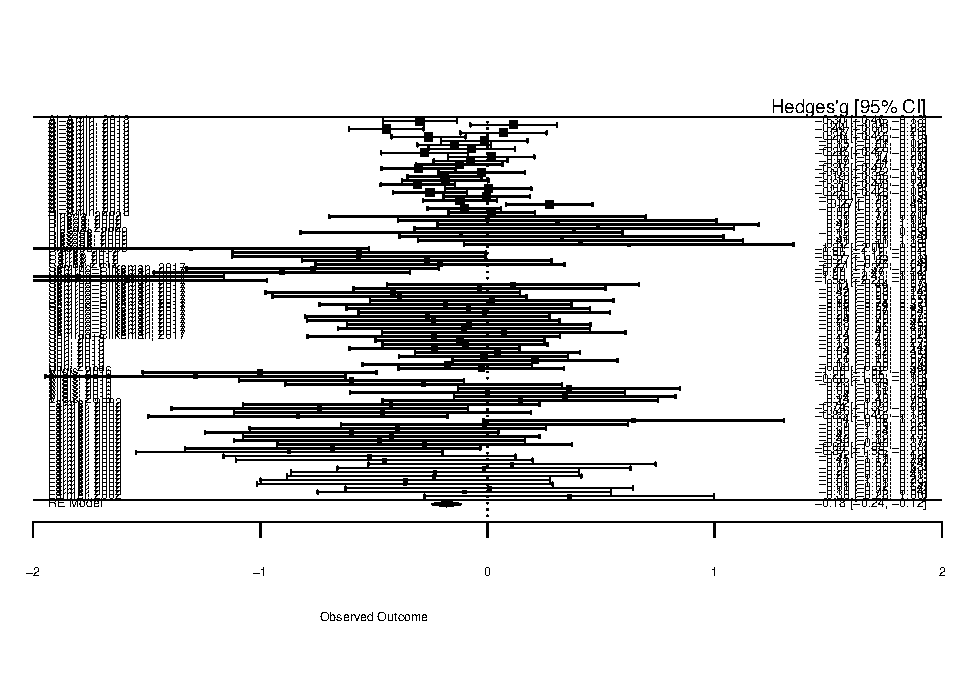
\includegraphics{_main_files/figure-latex/working-1.pdf}

\begin{Shaded}
\begin{Highlighting}[]
\FunctionTok{par}\NormalTok{(op)}
\end{Highlighting}
\end{Shaded}

\hypertarget{guerrilla-analytics-structure}{%
\chapter{Guerrilla analytics structure}\label{guerrilla-analytics-structure}}

The folder tree below shows my folder structure of the DAUR2 lessons. These lessons were are a part of the data science for biology 1 course.

\texttt{folder\ tree\ fs::dir\_tree(here::here("Guerrilla\_analytics\_framework",\ "Data\_daur2"))}

\hypertarget{curriculum-vitae}{%
\chapter{Curriculum vitae''}\label{curriculum-vitae}}

\hypertarget{personalia}{%
\subsection{Personalia}\label{personalia}}

Naam: Dian Dupon
Adres: \\
Telefoon: \\
E-mail: \href{mailto:dian.dupon@student.hu.nl}{\nolinkurl{dian.dupon@student.hu.nl}}
Geslacht: vrouw
Geboortedatum:
Nationaliteit: Nederlandse
Rijbewijs: Ja

\hypertarget{profiel}{%
\subsection{Profiel}\label{profiel}}

Ik ben een enthousiaste leerling. Bij het uitvoeren van een experiment ben ik altijd nieuwsgierig naar de uitslag. Dit motiveert mij dan ook om een zo goed en zo nauwkeurig mogelijke uitslag te krijgen. In de opleiding heb ik vaak te maken met deadlines. Hier kan ik goed mee omgaan.

\hypertarget{opleidingen}{%
\subsection{Opleidingen}\label{opleidingen}}

2020 -- 2024, Biologie en medisch laboratoriumonderzoek, HBO aan de Hogeschool Utrecht
2016 -- 2020, Biomedisch analist, MBO niveau 4 aan het Nova College te Beverwijk, diploma
2012 -- 2016, Saenredam College te Zaandijk, vmbo-tl, diploma

\hypertarget{werkervaring}{%
\subsection{Werkervaring}\label{werkervaring}}

Albert Heijn te Zaandam
Maart 2019 -- april 2023
Functiebenaming: medewerker vers

Expertisecentrum Leptospirose te Amsterdam
Januari 2020 -- juli 2020
Functiebenaming: stagiaire

Sanquin bloedvoorziening te Amsterdam
Augustus 2018 -- januari 2019
Functiebenaming: stagiaire

Dekamarkt te Zaandam
November 2016 -- december 2018
Functiebenaming: vakkenvuller

\hypertarget{vaardigheden}{%
\subsection{Vaardigheden}\label{vaardigheden}}

• (q)PCR
• MALDI-TOF MS
• VITEK2
• ELISA
• Western blot

  \bibliography{book.bib,packages.bib}

\end{document}
